\documentclass{article}
\usepackage{tmlr}

% --- Core packages -----------------------------------------------------------
\usepackage{amsmath,amssymb,amsfonts,amsthm}
\usepackage{mathtools}
\usepackage{microtype}
\usepackage{booktabs}
\usepackage{multirow}
\usepackage{array}
\usepackage{graphicx}
\usepackage{xcolor}
\usepackage{enumitem}
\usepackage{pifont}
\usepackage{url}
\usepackage[colorlinks=true,linkcolor=blue!70!black,citecolor=blue!70!black,urlcolor=blue!70!black]{hyperref}
\usepackage{natbib}

\renewcommand{\arraystretch}{1.10}

\theoremstyle{definition}
\newtheorem{definition}{Definition}
\newtheorem{proposition}{Proposition}

\newcommand{\cmark}{\textcolor{green!55!black}{\ding{51}}}
\newcommand{\xmark}{\textcolor{red!65!black}{\ding{55}}}
\newcommand{\Sres}{\mathcal{S}_{\text{res}}}
\newcommand{\Ssys}{\mathcal{S}_{\text{sys}}}
\newcommand{\beff}{b_{\text{eff}}}
\newcommand{\bpt}{\,bits/elem}

\title{Beyond Compression Ratio: Evaluating the Algorithmic\\ and Systems Utility of Long-Context\\ KV-Cache Compression\thanks{Large language models were used as assistive tools for stylistic editing and drafting under the authors' direct supervision. The authors take full responsibility for all content, experimental methodology, analysis, and scientific claims.}}

\author{\name Anonymous authors \\
        \addr Paper under double-blind review}

\begin{document}

\maketitle

% =============================================================================
\begin{abstract}
Key-value (KV) cache compression is almost always reported as a compression ratio paired with a task score. We show that this pairing is not sufficient to predict how a method will behave in a serving system, and that the two numbers do not even predict each other. Across 3{,}150 paired query executions spanning seven compression methods, three open-weight models (Gemma~4 E2B, Gemma~4 E4B, Qwen2.5~7B), five long-context tasks and context lengths from 2K to 128K tokens, we find that (i) at an \emph{identical} nominal budget of 4 bits per KV element, task accuracy ranges from 2.5\% to 47.3\% on Gemma~4 E2B --- an $18.7\times$ spread across methods that a compression ratio cannot distinguish; (ii) the memory a method saves carries essentially no information about the hardware efficiency it realises (Spearman $\rho = {+}0.04$, $p = 0.84$ over 36 operating points), and the compressed footprint carries none about prefill cost ($\rho = {+}0.01$, $p = 0.98$); and (iii) two methods matched to within 0.55 bits per element and 2.0 accuracy points differ by $30\times$ in time-to-first-token and $3.5\times$ in peak VRAM on the same model and prompts. Representation efficiency, task utility and serving efficiency are three separate axes, and a benchmark that collapses them hides exactly the information a practitioner needs.

We introduce CRBench, the measurement instrument these findings require: a query-level primitive that pairs every compressed execution with an uncompressed dense execution on the identical prompt, an effective-bits-per-element accounting that charges each representation for its mandatory metadata, and a decoupled two-track report separating algorithmic representation utility ($\Sres$) from measured serving utility ($\Ssys$). Charging for metadata is not a formality: it raises a factorised representation from a nominal 5.00 to a realised 6.51\bpt{} and a nominal 4-bit quantiser from 4.05 to 4.55\bpt{}, understatements of 30\% and 12\% that reorder the resulting table. We report per-method provenance, state which memory savings are physically realised and which are analytically accounted, and scope every conclusion to the models, implementations and hardware evaluated. Code, raw per-query records and the scripts that regenerate every number and figure are released.
\end{abstract}

% =============================================================================
\section{Introduction}
\label{sec:introduction}

Long-context inference is bounded by the key-value (KV) cache. Because standard attention caches key and value tensors for every past token at every layer and KV head, cache memory grows linearly in sequence length $L$ and batch size $B$:
\begin{equation}
\label{eq:kv_size}
M_{\text{KV}} = 2 \, N_{\text{layers}} \, N_{\text{kv heads}} \, d_{\text{head}} \, L \, B \cdot \text{sizeof}(\text{dtype}) \quad [\text{bytes}].
\end{equation}
For a Llama-3.1-8B-shaped model (32 layers, 8 KV heads under grouped-query attention, head dimension 128, 16-bit) a single 128K-token sequence needs $16.0$\,GiB for the cache alone --- more than the weights, and more than most consumer GPUs have. A large literature answers this with quantisation, token eviction, pooling, low-rank projection and factorised state~\citep{liu2024kivi,li2024snapkv,xiao2023streamingllm,zhang2023h2o,ge2023model,hooper2024kvquant}.

\paragraph{The reporting convention, and why it fails.}
These methods are almost universally summarised by two numbers: a compression ratio (or a nominal bit-width) and a task score. The implicit promise is that the first number tells you what the method costs and the second tells you what it costs you. Our measurements say otherwise, in three distinct ways.

\begin{figure}[t]
\centering
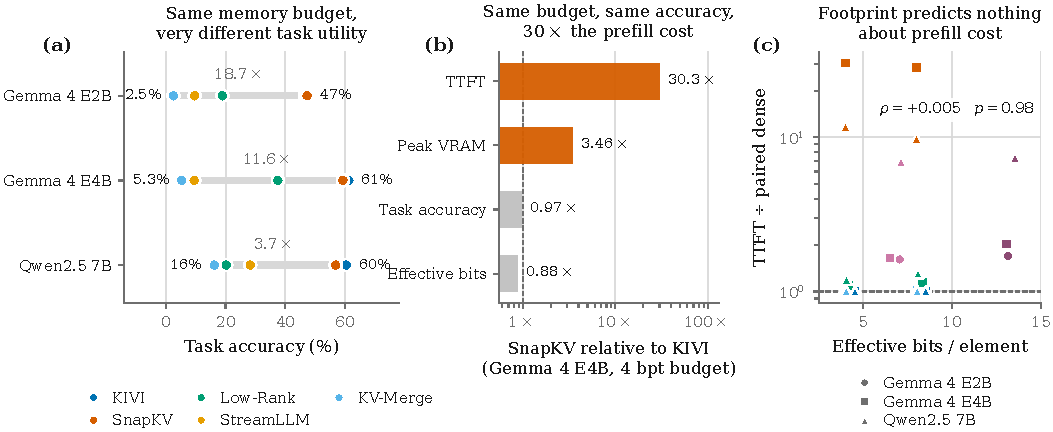
\includegraphics[width=\textwidth]{figures/fig1_decoupling.pdf}
\caption{\textbf{Three axes that do not substitute for one another.}
\textbf{(a)} Five methods held at an identical nominal budget of 4 bits per KV element --- realised payloads within $0.19$\bpt{} of one another, effective footprints within $0.55$ once metadata is charged --- differ in task accuracy by up to $18.7\times$. A compression ratio cannot tell these methods apart; only task measurement can.
\textbf{(b)} SnapKV and KIVI on Gemma~4 E4B agree to within 0.55 bits per element and 2.0 accuracy points, and then diverge by $3.5\times$ in peak VRAM and $30\times$ in time-to-first-token. Grey bars are the representation and quality axes; orange bars are the serving axis.
\textbf{(c)} Over all 36 compressed operating points, the effective footprint of a representation is uninformative about its prefill cost. Marker shape denotes model, colour denotes method.
Panel (b) reflects the SnapKV integration described in \S\ref{sec:provenance}, not SnapKV's fused reference kernel.}
\label{fig:decoupling}
\end{figure}

\emph{First, the compression ratio does not determine task utility.} Figure~\ref{fig:decoupling}(a) holds five methods at the same nominal 4-bit budget --- their realised payloads agree to within $0.19$ bits per element, and their effective footprints to within $0.55$ --- and finds accuracy spanning $2.5\%$ to $47.3\%$ on Gemma~4 E2B, $5.3\%$ to $61.3\%$ on Gemma~4 E4B, and $16.2\%$ to $60.4\%$ on Qwen2.5~7B. Pooled over all 36 compressed operating points in our study, the rank correlation between memory saved and accuracy achieved is $\rho = {-}0.42$ ($p = 0.010$): saving more memory is, if anything, associated with retaining \emph{less} task ability. A compression ratio reported without a task measurement is close to uninformative.

\emph{Second, the task score does not determine serving behaviour.} Figure~\ref{fig:decoupling}(b) takes two methods that agree on both of the reported numbers --- within $0.55$ bits per element and $2.0$ accuracy points on the same model and the same prompts --- and shows them diverging by $3.46\times$ in peak VRAM and $30.3\times$ in time-to-first-token (TTFT). Nothing in the conventional report anticipates this. Over all operating points, memory saved has no rank relationship to the measured hardware efficiency multiplier ($\rho = {+}0.04$, $p = 0.84$), and the effective footprint has none to prefill cost ($\rho = {+}0.01$, $p = 0.98$) or to measured peak VRAM ($\rho = {-}0.08$, $p = 0.63$).

\emph{Third, the compression ratio is usually misreported.} A representation's real cost is its payload \emph{plus} the metadata that makes the payload decodable: quantisation scales and zero points, codebooks, subspace bases, eviction index tables. Charging for that metadata moves a factorised representation from a nominal $5.00$ to a realised $6.51$ bits per element, and a nominal 4-bit quantiser from $4.05$ to $4.55$ --- understatements of $30\%$ and $12\%$, in the direction that flatters the method. Because the overhead is concentrated in particular method families rather than spread evenly, correcting it also reorders the ranking.

\paragraph{What follows.}
The rest of the paper takes these three findings seriously as a measurement problem. \S\ref{sec:axes} states the three axes precisely and argues why none is recoverable from the others. \S\ref{sec:crbench} develops CRBench, the instrument that measures them jointly: a query-level primitive that runs every compressed configuration against a dense reference on the identical prompt, an effective-bits accounting that charges for metadata, and two reported scores that are deliberately not merged into one. \S\ref{sec:setup} and \S\ref{sec:results} give the study and its results, organised around the three questions above. \S\ref{sec:discussion} draws out what this means for method authors and practitioners, and \S\ref{sec:limitations} is explicit about what our evidence does and does not support.

\paragraph{Contributions.}
\begin{itemize}[leftmargin=*,itemsep=2.0pt,topsep=3pt]
    \item \textbf{An empirical separation of three axes that the field reports as two.} At matched nominal bitrates, task accuracy varies by up to $18.7\times$; at matched bitrate \emph{and} matched accuracy, serving cost varies by $30\times$. We quantify the (near-zero) rank association between representation footprint and realised hardware behaviour across 36 operating points and three models.
    \item \textbf{Effective bits per element ($\beff$), an accounting that charges for metadata.} We show it is not a bookkeeping detail: it changes reported bitrates by $6$--$28\%$ depending on the method family, and it penalises exactly the methods that carry auxiliary state. Applied honestly, it demotes configurations we might otherwise have highlighted.
    \item \textbf{A decoupled two-track report ($\Sres$, $\Ssys$) with an auditable dense pairing.} Every query is executed twice on the identical prompt, once dense and once compressed, and both outcomes are logged; coverage is reported alongside the scores rather than folded into them.
    \item \textbf{A study designed for interpretability rather than a leaderboard.} 3{,}150 paired executions over 75 distinct queries per model, at two controlled bit budgets, with per-method provenance stating which implementation was used and whether its savings were physically realised or analytically accounted.
\end{itemize}

% =============================================================================
\section{Three Axes, and Why They Do Not Substitute}
\label{sec:axes}

We distinguish three properties of a KV-cache compression method that the literature routinely conflates.

\paragraph{Axis 1: representation efficiency.} How many bits of state the method actually keeps per KV element, including everything needed to decode that state. This is a property of the representation alone. It is what a compression ratio is trying to express, and it is what determines how much longer a context fits in a fixed memory budget.

\paragraph{Axis 2: task utility.} How much of the model's task ability survives the transform, measured on the same prompts against the same dense reference. This is a property of the representation \emph{and} the model \emph{and} the task.

\paragraph{Axis 3: serving efficiency.} What the method costs in wall-clock prefill latency, decode throughput and resident device memory when actually executed. This is a property of the representation, its \emph{implementation}, and the hardware.

\paragraph{Why Axis 1 does not give Axis 2.} Two representations can retain the same number of bits and spend them completely differently. A 4-bit quantiser spends its budget uniformly across all tokens; an eviction policy spends 16 bits on a quarter of the tokens and nothing on the rest; a pooling scheme spends them on averages that may not correspond to any token the model needs. Which allocation is right depends on where the task's information lies, which the bit count cannot express. \S\ref{sec:res_axis12} measures the resulting spread.

\paragraph{Why Axis 1 does not give Axis 3, in four concrete ways.}
\begin{enumerate}[leftmargin=*,itemsep=2.0pt,topsep=3pt]
    \item \textbf{Metadata is not free and is not proportional.} Group-wise quantisation must store a scale and zero point per group; a factorised scheme must store anchors and subspace bases; an eviction method needs only a position index. At a nominal 4-bit budget these carry overheads of $11\%$, $23\%$ and $0.1\%$ of realised footprint respectively in our measurements (\S\ref{sec:res_metadata}). A ratio computed on payload alone therefore mis-ranks them.
    \item \textbf{Prefill cost is decided by the transform, not the footprint.} A method that reduces resident memory can still add an expensive pass over the prompt. Attention-score pooling, SVD and block factorisation all do work proportional to the \emph{uncompressed} prompt before any saving materialises. Our measured TTFT inflation ranges from $0.96\times$ to $30.3\times$ dense at effectively identical footprints.
    \item \textbf{Implementation efficiency is part of the answer.} The same algorithm, expressed as a fused kernel or as un-fused tensor operations, is a different serving proposition. This is not a defect of the measurement --- it is the quantity a practitioner is actually choosing between, and it cannot be read off a paper's compression ratio.
    \item \textbf{Peak memory is not resident memory.} A transform that ends up smaller can pass through a much larger intermediate. In our runs the method with the smallest analytic footprint at 4 bits also had the largest measured peak VRAM, $3.5\times$ the alternative.
\end{enumerate}

\noindent The practical consequence is that the three axes must be measured, separately, on the same queries. That is what CRBench is for.

% =============================================================================
\section{Related Work}
\label{sec:related}

\paragraph{Long-context evaluation.} Needle-in-a-Haystack~\citep{kamradt2023needle}, RULER~\citep{hsieh2024ruler}, LongBench~\citep{bai2023longbench,bai2024longbenchv2}, L-Eval~\citep{an2023leval}, BAMBOO~\citep{dong2023bamboo} and $\infty$-Bench~\citep{zhang2024infinitebench} measure what a model can do with a long context. They do not track what that context costs, and they evaluate uncompressed models, so they cannot separate a representation's contribution from the base model's.

\paragraph{Compression methods.} KIVI~\citep{liu2024kivi}, KVQuant~\citep{hooper2024kvquant} and LLM.int8()~\citep{dettmers2022llmint8} quantise; SnapKV~\citep{li2024snapkv}, StreamingLLM~\citep{xiao2023streamingllm}, $\text{H}_2\text{O}$~\citep{zhang2023h2o} and Scissorhands~\citep{liu2023scissorhands} evict; \citet{ge2023model} and PyramidKV~\citep{zhang2024pyramidkv} merge or allocate adaptively; low-rank approaches project~\citep{sharma2023truth}. Each reports on its own task subset, at its own bit accounting, on its own hardware, typically against a baseline reproduced by its own authors. The literature is therefore rich in individually credible results that cannot be placed on a common axis.

\paragraph{Systems measurement.} Serving stacks report latency, throughput and memory but not task quality, and generally not per representation. The gap we address is not that any one of these communities measures badly; it is that the three measurements are never taken on the same queries, so their disagreements are invisible.

\begin{table}[t]
\centering
\small
\setlength{\tabcolsep}{4.5pt}
\caption{What existing evaluation practice records. ``Dense anchor'' means an uncompressed run of the \emph{same} model is reported; ``paired'' means that run is on the \emph{same} query. $\triangle$ = sometimes, inconsistently.}
\label{tab:paradigms}
\begin{tabular}{lccccc}
\toprule
\textbf{Evaluation practice} & \textbf{Task quality} & \textbf{Memory} & \textbf{Latency} & \textbf{Dense anchor} & \textbf{Paired} \\
\midrule
Long-context suites (LongBench, L-Eval) & \cmark & \xmark & \xmark & \xmark & \xmark \\
Synthetic probes (NIAH, RULER) & \cmark & \xmark & \xmark & \xmark & \xmark \\
Serving-system profilers & \xmark & \cmark & \cmark & \xmark & \xmark \\
Compression method papers & \cmark & $\triangle$ & $\triangle$ & $\triangle$ & \xmark \\
\textbf{CRBench (this work)} & \cmark & \cmark & \cmark & \cmark & \cmark \\
\bottomrule
\end{tabular}
\end{table}

% =============================================================================
\section{CRBench: Measuring the Three Axes Jointly}
\label{sec:crbench}

\subsection{The paired query primitive}

Let $\mathcal{M}$ be an autoregressive model with fixed weights, $\mathcal{D} = \{(x_i, y_i, \tau_i, L_i)\}_{i=1}^N$ a dataset of queries with targets, task types and context lengths, $\mathcal{R}_{\text{dense}}$ the uncompressed 16-bit reference representation, and $\mathcal{A}(\mathcal{B})$ a candidate representation under budget $\mathcal{B}$.

\begin{definition}[Paired evaluation unit]
\label{def:unit}
The atomic unit of CRBench is the 4-tuple $\mathcal{U}_i = (\mathcal{M},\, (x_i,y_i),\, \mathcal{R}_{\text{dense}},\, \mathcal{A}(\mathcal{B}))$. For each unit CRBench executes the dense reference $\hat{y}_{i,\text{dense}} = \mathcal{M}(x_i \mid \mathcal{R}_{\text{dense}})$ and the candidate $\hat{y}_{i,\text{method}} = \mathcal{M}(x_i \mid \mathcal{A}(\mathcal{B}))$ on the identical prompt, and records for both: the task score $s \in [0,1]$, the analytic state footprint in bytes, and the measured TTFT, decode throughput and peak device memory.
\end{definition}

Pairing at the query level rather than the dataset level is what makes the three axes comparable. Every ratio we report --- accuracy retention, TTFT inflation, VRAM inflation --- is formed against a dense execution of the same prompt in the same session, so it cannot be contaminated by a differently configured or differently reported baseline.

\subsection{Task quality}

\begin{definition}[Absolute task quality]
For a completed candidate run with evaluator score $s_{i,\text{method}} \in [0,1]$,
\begin{equation}
\label{eq:quality}
Q_{\text{abs},i} = 100 \cdot \min\!\big(1, \max(0,\, s_{i,\text{method}})\big).
\end{equation}
\end{definition}

We deliberately report absolute success rather than retention relative to dense. Retention rewards a method for being paired with a weak baseline: a method that scores $20\%$ where dense scores $20\%$ has $100\%$ retention and is useless. The paired dense outcome is still recorded for every query --- it defines coverage, enables failure diagnosis, and lets a reader recompute retention where a task has a defensible chance floor --- but it is not substituted into the headline number. We log the signed paired difference $\Delta_i = s_{i,\text{method}} - s_{i,\text{dense}}$ throughout.

\subsection{Memory accounting: effective bits per element}
\label{sec:beff}

This is the axis most often misreported, so we make the accounting explicit. For any representation the total state is
\begin{equation}
\label{eq:memory}
M_{\text{method}}(L) = \underbrace{M_{\text{algo}}(L)}_{\text{compressed payload}} + \underbrace{M_{\text{meta}}(L)}_{\text{scales, zero points, codebooks, bases, index tables}} + \underbrace{M_{\text{align}}(L)}_{\text{padding}} \quad [\text{bytes}].
\end{equation}

\begin{definition}[Effective bits per element]
\label{def:beff}
Normalising the \emph{total} state by the uncompressed KV element count,
\begin{equation}
\label{eq:beff}
\beff = \frac{8 \cdot M_{\text{method}}(L)}{2 \, N_{\text{layers}} \, N_{\text{kv heads}} \, d_{\text{head}} \, L} \quad [\text{bits/element}],
\end{equation}
which is exactly $16.0$ for an uncompressed FP16/BF16 cache.
\end{definition}

\paragraph{Why the metadata term is load-bearing.} A method's nominal bit-width describes only $M_{\text{algo}}$. The remaining terms are not optional: without the scales, the quantised payload cannot be dequantised; without the bases, the projection cannot be inverted. They are also not uniform across method families --- group-wise quantisation pays per group, a subspace method pays per block, and an eviction method pays only a token index --- so omitting them does not merely shift every method equally, it \emph{re-ranks} them. \S\ref{sec:res_metadata} quantifies this at $6$--$28\%$ of realised footprint depending on the method.

\begin{definition}[Memory saving]
$R_{\text{mem},i} = 100 \cdot \max\!\big(0,\, 1 - M_{i,\text{method}} / M_{i,\text{dense}}\big) \in [0,100]$.
\end{definition}

\paragraph{Analytic versus physically realised savings.} We distinguish two things a compression result can mean. A saving is \emph{physically realised} when the resident cache tensors actually shrink, and \emph{analytically accounted} when the scheme's footprint is computed from its definition while the harness keeps the transformed values in a wider dtype for exactness. Both are legitimate --- the first measures a system, the second measures a representation --- but they are not interchangeable, and conflating them is how a paper ends up claiming a serving win it did not measure. \S\ref{sec:provenance} states which is which for every method here, and peak-VRAM measurements in the Part~2 track always reflect what was physically resident.

\subsection{Part 1: algorithmic representation utility}

\begin{equation}
\label{eq:sres}
\Sres = \alpha \, Q_{\text{abs}} + (1 - \alpha)\, R_{\text{mem}}, \qquad \alpha = 0.70 \text{ by default}.
\end{equation}
The linear form is chosen for transparency, not optimality: it is monotone in both arguments, bounded on $[0,100]$, Pareto consistent, and --- unlike a product or harmonic form --- never lets one dimension annihilate the other, so a reader can always decompose a score back into the two quantities that produced it (proof in Appendix~\ref{app:proofs}; comparison with multiplicative alternatives in Appendix~\ref{app:formulations}). At $\alpha = 0.70$ one accuracy point is worth $2.33$ points of memory saving. We report $\alpha$ sensitivity in Figure~\ref{fig:alpha} rather than asking the reader to accept the default; the qualitative ordering is stable over $\alpha \in [0.4, 0.9]$.

Aggregation over a dataset uses the arithmetic mean of $Q_{\text{abs}}$ and a byte-weighted aggregate of memory, $\bar{R}_{\text{mem}} = 100(1 - \sum_i M_{i,\text{method}} / \sum_i M_{i,\text{dense}})$, so that long contexts --- where compression matters --- are not diluted by short ones. Failed queries are charged the dense footprint and score zero rather than being dropped.

\paragraph{Coverage is reported, not folded in.} We report paired coverage $C_{\text{paired}} = N_{\text{paired success}} / N_{\text{total}}$ beside $\Sres$ as a pair $(\Sres, C_{\text{paired}})$ rather than multiplying it in, so that a run that failed for allocator reasons is visibly distinguishable from a run that completed and scored zero. Coverage was $1.00$ for every configuration reported here.

\subsection{Part 2: measured serving utility}
\label{sec:part2}

Part~2 records TTFT (wall-clock to first emitted token, including all transform work), decode throughput $\mathcal{T}_{\text{dec}}$ in tokens/s, and peak resident device memory $\mathcal{M}_{\text{peak}}$. Each is converted to a paired efficiency against the \emph{same query's} dense execution:
\begin{equation}
\label{eq:phi_components}
\phi_{\text{ttft}} = \min\!\Big(1, \tfrac{\text{TTFT}_{\text{dense}}}{\text{TTFT}_{\text{method}}}\Big),\quad
\phi_{\text{thru}} = \min\!\Big(1, \tfrac{\mathcal{T}_{\text{method}}}{\mathcal{T}_{\text{dense}}}\Big),\quad
\phi_{\text{vram}} = \min\!\Big(1, \tfrac{\mathcal{M}_{\text{dense}}}{\mathcal{M}_{\text{method}}}\Big),
\end{equation}
combined into a hardware multiplier and a system score
\begin{equation}
\label{eq:phi}
\phi = \phi_{\text{ttft}}^{0.35}\, \phi_{\text{thru}}^{0.35}\, \phi_{\text{vram}}^{0.30}, \qquad R_{\text{sys}} = 100\phi, \qquad \Ssys = \alpha \Sres + (1-\alpha) R_{\text{sys}}.
\end{equation}
The weights give interactive responsiveness (TTFT and decode, $0.35$ each) slightly more emphasis than resident footprint ($0.30$); we make no claim that this is the only defensible weighting, and the components are always reported separately so a reader can reweight. $\phi$ is computed per query and then averaged; the TTFT, throughput and VRAM values in our tables are descriptive means and are not substituted back into Equation~\ref{eq:phi}.

\paragraph{$\Ssys$ is a summary, not evidence.} Because $\Ssys$ contains $\Sres$ by construction, a correlation between them is circular and we never use one. Where we ask whether algorithmic utility predicts serving behaviour we correlate against $\phi$, the pure hardware term.

\begin{figure}[t]
\centering
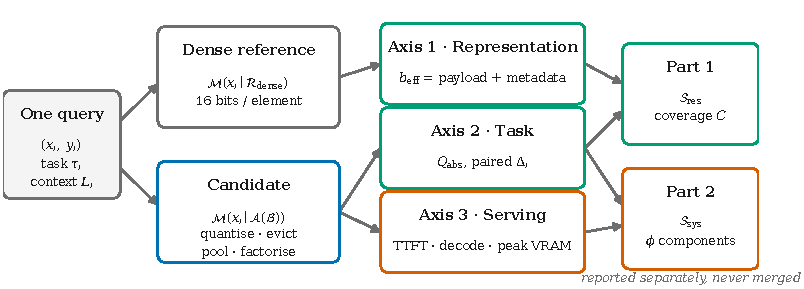
\includegraphics[width=0.95\textwidth]{figures/fig2_framework.pdf}
\caption{\textbf{CRBench measurement flow.} A single query is executed twice on the identical prompt --- once under the dense reference, once under the candidate representation --- and the two executions are compared on all three axes. Part~1 ($\Sres$) reports the representation; Part~2 ($\Ssys$) reports what the representation cost on the hardware it ran on. The tracks are reported separately by design.}
\label{fig:framework}
\end{figure}

% =============================================================================
\section{Experimental Setup}
\label{sec:setup}

\subsection{Design}

Each model is evaluated on $5$ tasks $\times$ $5$ context lengths $\times$ $3$ samples $= 75$ distinct queries. Each query is executed under $14$ configurations: five fixed-budget methods at nominal budgets of $4$ and $8$ bits per element, two adaptive DKV configurations, and the dense reference (recorded in both budget sweeps). This gives $1{,}050$ paired executions per model and $3{,}150$ in total. Decoding is greedy ($T=0$); the generation budget is fixed per task ($32$--$256$ new tokens) and identical across every configuration, so no method is advantaged by a longer or shorter budget.

Reporting operating points separately, rather than pooling the two budget sweeps into one row per method, is deliberate: a pooled ``$\approx\!6$ bits'' row averages two configurations whose accuracies can differ by more than $30$ points, and it is precisely the matched-budget comparison that carries the paper's evidence.

\subsection{Models and context ladders}
\begin{itemize}[leftmargin=*,itemsep=1.0pt,topsep=2pt]
    \item \textbf{Gemma~4 E2B} (\texttt{google/gemma-4-e2b-it}): $2$K, $8$K, $32$K, $64$K, $128$K.
    \item \textbf{Gemma~4 E4B} (\texttt{google/gemma-4-e4b-it}): $2$K, $4$K, $8$K, $16$K, $32$K.
    \item \textbf{Qwen2.5~7B} (\texttt{Qwen/Qwen2.5-7B-Instruct}): $2$K, $4$K, $8$K, $16$K, $32$K.
\end{itemize}

\subsection{Tasks}
Single-needle and multi-needle retrieval at parameterised depths; RULER key--value lookup among distractors~\citep{hsieh2024ruler}; RULER multi-step variable tracking~\citep{hsieh2024ruler}; and synthetic cross-document multi-hop QA. Two of the five behave as controls rather than discriminators in our study and we treat them as such in \S\ref{sec:res_tasks}.

\subsection{Environment}
All runs were executed on a single NVIDIA GeForce RTX 4070 SUPER ($12$\,GB VRAM), with PyTorch $2.6.0$ (CUDA 12.4 build), \texttt{transformers} $5.15.1$ and Python $3.12.10$ on Windows 11. Model weights were loaded in 4-bit NormalFloat (NF4) via bitsandbytes so that the weight footprint is held constant and the $128$K ladder fits in $12$\,GB; the KV cache under study is unaffected by this choice. Prefill used chunked forward passes ($4{,}096$ tokens) to avoid intermediate allocation spikes. Because every comparison is paired against a dense execution on the same device in the same session, absolute latencies are hardware-specific but the reported ratios are not distorted by machine-to-machine variation.

\paragraph{Determinism.} The dense reference was executed twice for every query, once in each budget sweep. On Gemma~4 E4B and Qwen2.5~7B all $150$ re-executions produced byte-identical outputs. On Gemma~4 E2B, $64/75$ produced identical text and exactly one query changed score --- a multi-needle prompt at $128$K. Run-to-run variance is therefore negligible at the resolution of our claims, and is smallest where the claims are strongest.

\subsection{Methods and provenance}
\label{sec:provenance}

Table~\ref{tab:provenance} states, for every method, which implementation produced the numbers and whether its memory saving was physically realised or analytically accounted. We consider this disclosure part of the result rather than an appendix detail: a serving claim is only as strong as the code path that produced it.

\begin{table}[t]
\centering
\small
\setlength{\tabcolsep}{3.6pt}
\caption{\textbf{Per-method provenance.} ``Upstream'' means the authors' own released code was invoked; ``CRBench'' means a reference implementation written for this harness following the published scheme. ``Realised'' means the resident cache tensors physically shrank; ``analytic'' means the footprint was computed from the scheme while values were retained in a wider dtype, so quality is exact for the scheme but no device memory was freed.}
\label{tab:provenance}
\begin{tabular}{@{}l l l l >{\raggedright\arraybackslash}p{7.1cm}@{}}
\toprule
\textbf{Method} & \textbf{Impl.} & \textbf{Saving} & \textbf{Budget} & \textbf{Notes} \\
\midrule
KIVI (INT4/INT8) & CRBench & analytic & 4, 8 & Asymmetric grouped min--max, per-channel keys and per-token values, following \citet{liu2024kivi}. Partial key groups stay at 16 bits and are charged as such. \\[2pt]
SnapKV & Upstream & realised & 4, 8 & \texttt{SnapKVCluster.update\_kv} at \texttt{e216ddc}. Upstream's monkeypatch targets \texttt{transformers}~4.37 and Llama/Mistral only, so under \texttt{transformers}~5.x the cluster is driven directly, \emph{outside} the fused attention path. \\[2pt]
StreamingLLM & Upstream & realised & 4, 8 & \texttt{StartRecentKVCache} at \texttt{2e50426}; policy unmodified. \\[2pt]
KV-Merging & CRBench & realised & 4, 8 & Temporal mean-pooling of consecutive states, sinks and recent window preserved~\citep{ge2023model}. \\[2pt]
Low-Rank KV & CRBench & analytic & 4, 8 & Per-head mean-centred truncated SVD~\citep{sharma2023truth}; footprint is the $U,\Sigma,V$ factor size. \\[2pt]
DKV-Mid / High & Upstream & analytic & adaptive & Anchor-plus-low-rank differential compression. The block compressor is driven over the resident cache; the repository's paged serving runtime and Triton decode kernel were unavailable on this platform, so these numbers characterise the representation, \emph{not} that runtime's decode speedup. \\[2pt]
Dense FP16 & --- & --- & 16 & Uncompressed reference. \\
\bottomrule
\end{tabular}
\end{table}

\paragraph{On SnapKV in particular.} The prefill cost we measure for SnapKV is a property of this integration, not of SnapKV as published: driven outside its fused attention path, the observation-window pooling runs as separate tensor operations over the full prompt. We report it because it is the honest measurement of the code path that was runnable here, and because it illustrates the paper's own thesis --- serving efficiency is a property of an algorithm \emph{and} its implementation, and is therefore not predictable from the algorithm's compression ratio. It should not be read as a claim about SnapKV's achievable latency. The same caveat, in the opposite direction, applies to DKV: its representation is measured, its serving runtime is not.

% =============================================================================
\section{Results}
\label{sec:results}

\subsection{Does the compression ratio predict task utility? No.}
\label{sec:res_axis12}

Table~\ref{tab:part1} reports every operating point. Reading across a fixed nominal budget isolates Axis~1 from Axis~2: the five fixed-budget methods at $4$ bits realise payloads within $0.19$ bits per element of one another, and effective footprints within $0.55$ once metadata is charged, so any accuracy difference between them is attributable to \emph{how} they spend the budget rather than how much they spend.

The differences are large. On Gemma~4 E2B accuracy at $4$ bits ranges from $2.5\%$ (KV-Merging) to $47.3\%$ (SnapKV), a factor of $18.7$; on Gemma~4 E4B from $5.3\%$ to $61.3\%$ ($11.6\times$); on Qwen2.5~7B from $16.2\%$ to $60.4\%$ ($3.7\times$). At $8$ bits the spreads narrow but remain substantial ($22.2$, $21.2$ and $37.4$ accuracy points respectively), because the methods that fail at $4$ bits recover unevenly: StreamingLLM gains $26.5$ points on E2B between the two budgets while KIVI gains none ($46.7\% \to 46.2\%$, within noise). How much accuracy a bit buys is itself method-dependent.

Pooled over all $36$ compressed operating points, the rank correlation between memory saved and accuracy is $\rho = {-}0.42$ ($p = 0.010$); per model it is ${-}0.28$, ${-}0.64$ and ${-}0.39$. The negative sign is unsurprising --- within a method family, saving more costs accuracy --- but the point is the absence of any positive predictive relationship \emph{across} methods. A reader given only a compression ratio cannot order these methods on task ability, even approximately.

\begin{table}[t]
\centering
\small
\setlength{\tabcolsep}{5.0pt}
\caption{\textbf{Part 1: algorithmic representation utility at every operating point.} $b_{\text{pay}}$ is the compressed payload alone --- the quantity conventionally reported --- and $\beff$ additionally charges mandatory metadata (Definition~\ref{def:beff}); ``meta'' is the metadata share of realised footprint. $\Sres = 0.70\,Q_{\text{abs}} + 0.30\,R_{\text{mem}}$ on $\beff$. Best $\Sres$ per model in \textbf{bold}. Paired coverage was $1.00$ throughout.}
\label{tab:part1}
\begin{tabular}{ll ccc c c}
\toprule
\textbf{Method} & \textbf{Budget} & \textbf{Accuracy} & $b_{\text{pay}}$ & $b_{\text{eff}}$ & \textbf{meta} & $\mathcal{S}_{\text{res}}$ \\
\midrule
\multicolumn{7}{l}{\textit{Gemma 4 E2B (2K--128K)}} \\
\midrule
KIVI (INT4/INT8) & 4 & 46.7\% & 4.01 & 4.51 & 11.1\% & 54.2 \\
KIVI (INT4/INT8) & 8 & 46.2\% & 8.01 & 8.51 & 5.9\% & 46.4 \\
SnapKV & 4 & 47.3\% & 4.00 & 4.01 & 0.2\% & \textbf{55.6} \\
SnapKV & 8 & 46.2\% & 8.00 & 8.02 & 0.2\% & 47.3 \\
Low-Rank KV & 4 & 18.9\% & 4.05 & 4.05 & 0.0\% & 35.7 \\
Low-Rank KV & 8 & 43.6\% & 8.09 & 8.09 & 0.0\% & 45.3 \\
StreamingLLM & 4 & 9.6\% & 4.00 & 4.01 & 0.2\% & 29.2 \\
StreamingLLM & 8 & 36.1\% & 8.00 & 8.02 & 0.2\% & 40.2 \\
KV-Merging & 4 & 2.5\% & 4.01 & 4.02 & 0.4\% & 24.2 \\
KV-Merging & 8 & 24.0\% & 8.01 & 8.04 & 0.4\% & 31.7 \\
DKV-Mid & adaptive & 44.7\% & 5.46 & 7.07 & 22.8\% & 48.0 \\
DKV-High & adaptive & 46.7\% & 10.78 & 13.17 & 18.1\% & 38.0 \\
Dense FP16 & -- & 46.4\% & 16.00 & 16.00 & 0.0\% & 32.5 \\
\midrule
\multicolumn{7}{l}{\textit{Gemma 4 E4B (2K--32K)}} \\
\midrule
KIVI (INT4/INT8) & 4 & 61.3\% & 4.05 & 4.55 & 10.9\% & \textbf{64.4} \\
KIVI (INT4/INT8) & 8 & 62.7\% & 8.03 & 8.53 & 5.8\% & 57.9 \\
SnapKV & 4 & 59.3\% & 4.00 & 4.00 & 0.1\% & 64.0 \\
SnapKV & 8 & 60.7\% & 8.00 & 8.01 & 0.1\% & 57.5 \\
Low-Rank KV & 4 & 37.5\% & 4.19 & 4.19 & 0.0\% & 48.4 \\
Low-Rank KV & 8 & 60.0\% & 8.34 & 8.34 & 0.0\% & 56.4 \\
StreamingLLM & 4 & 9.5\% & 4.00 & 4.00 & 0.1\% & 29.1 \\
StreamingLLM & 8 & 41.4\% & 8.00 & 8.01 & 0.1\% & 44.0 \\
KV-Merging & 4 & 5.3\% & 4.03 & 4.04 & 0.2\% & 26.1 \\
KV-Merging & 8 & 45.3\% & 8.02 & 8.04 & 0.2\% & 46.7 \\
DKV-Mid & adaptive & 55.3\% & 5.00 & 6.51 & 23.2\% & 56.5 \\
DKV-High & adaptive & 61.3\% & 10.68 & 13.07 & 18.3\% & 48.4 \\
Dense FP16 & -- & 64.0\% & 16.00 & 16.00 & 0.0\% & 44.8 \\
\midrule
\multicolumn{7}{l}{\textit{Qwen2.5 7B (2K--32K)}} \\
\midrule
KIVI (INT4/INT8) & 4 & 60.4\% & 4.05 & 4.55 & 10.9\% & \textbf{63.8} \\
KIVI (INT4/INT8) & 8 & 60.9\% & 8.04 & 8.53 & 5.8\% & 56.6 \\
SnapKV & 4 & 56.9\% & 4.00 & 4.01 & 0.2\% & 62.3 \\
SnapKV & 8 & 59.6\% & 8.00 & 8.02 & 0.2\% & 56.7 \\
Low-Rank KV & 4 & 20.2\% & 4.07 & 4.07 & 0.0\% & 36.5 \\
Low-Rank KV & 8 & 36.9\% & 8.10 & 8.10 & 0.0\% & 40.6 \\
StreamingLLM & 4 & 28.3\% & 4.00 & 4.01 & 0.2\% & 42.3 \\
StreamingLLM & 8 & 44.8\% & 8.00 & 8.02 & 0.2\% & 46.3 \\
KV-Merging & 4 & 16.2\% & 4.03 & 4.05 & 0.4\% & 33.8 \\
KV-Merging & 8 & 23.5\% & 8.02 & 8.05 & 0.4\% & 31.4 \\
DKV-Mid & adaptive & 53.3\% & 5.84 & 7.15 & 18.3\% & 53.9 \\
DKV-High & adaptive & 59.1\% & 12.14 & 13.55 & 10.4\% & 46.0 \\
Dense FP16 & -- & 60.0\% & 16.00 & 16.00 & 0.0\% & 42.0 \\
\bottomrule
\end{tabular}

\end{table}

\subsection{How much does metadata cost? Six to twenty-eight percent.}
\label{sec:res_metadata}

Figure~\ref{fig:effective_bits} decomposes each operating point into payload and mandatory metadata. The overhead is heavily method-dependent. Eviction and pooling methods store only a token index and pay $0.1$--$0.4\%$. Grouped quantisation pays for scales and zero points: a nominal $4$-bit configuration realises $4.51$--$4.55$ bits per element ($11\%$ overhead), and because the metadata is per group rather than per bit, the same scheme at $8$ bits pays only $5.8$--$5.9\%$. The factorised DKV representations pay most: $18$--$23\%$, moving DKV-Mid from a nominal $5.00$ to a realised $6.51$ bits per element on Gemma~4 E4B, and DKV-High from $10.68$ to $13.07$ --- at which point it is saving $18\%$ of the dense footprint rather than the $33\%$ a payload-only accounting would report.

This matters for ranking, not only for absolute numbers. Because the overhead is concentrated in one method family, charging for it reorders the table: on Gemma~4 E4B, DKV-Mid falls from third to fifth of thirteen operating points, passed by both 8-bit configurations it had outranked; on Gemma~4 E2B and Qwen2.5~7B, DKV-High falls one position, passed by 8-bit StreamingLLM. The eviction and pooling methods are untouched, because they had almost nothing to be charged for. We note that DKV is the representation family for which this correction is largest, and applying it costs that family rank positions in our own tables; it does not, on this suite, push any DKV configuration below the uncompressed dense reference.

\begin{figure}[t]
\centering
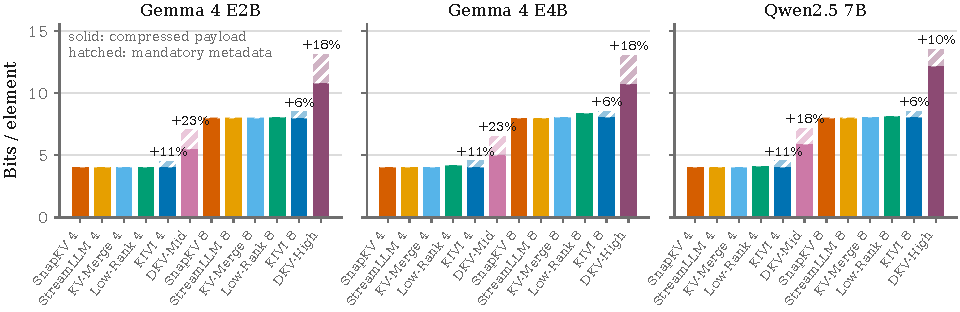
\includegraphics[width=\textwidth]{figures/fig4_effective_bits.pdf}
\caption{\textbf{Nominal payload versus effective bits per element.} Solid bars are the compressed payload conventionally reported as the compression ratio; hatched caps are the mandatory metadata that makes the payload decodable. Labels give the metadata share where it exceeds $5\%$. Eviction methods carry almost none; grouped quantisation carries $6$--$11\%$; factorised representations carry $18$--$23\%$.}
\label{fig:effective_bits}
\end{figure}

\subsection{Does task utility predict serving efficiency? No.}
\label{sec:res_axis23}

Table~\ref{tab:part2} reports the measured serving track. The clearest evidence is a matched pair. On Gemma~4 E4B at a $4$-bit budget, KIVI and SnapKV agree closely on both conventionally reported numbers --- $4.55$ versus $4.00$ bits per element, $61.3\%$ versus $59.3\%$ accuracy --- and then diverge completely on the third axis: TTFT of $2.84$\,s versus $86.04$\,s ($30.3\times$), peak VRAM of $761$\,MB versus $2{,}632$\,MB ($3.46\times$), hardware multiplier $\phi$ of $0.99$ versus $0.48$, and $\Ssys$ of $74.7$ versus $59.1$. The same pair on Qwen2.5~7B differs by $11.7\times$ in TTFT. Nothing in Axis~1 or Axis~2 anticipates a $30\times$ latency gap.

Across all operating points the association is absent rather than merely weak. Memory saved has no rank relationship to the measured hardware multiplier ($\rho = {+}0.04$, $p = 0.84$); effective footprint has none to TTFT inflation ($\rho = {+}0.01$, $p = 0.98$) or to measured peak-VRAM inflation ($\rho = {-}0.08$, $p = 0.63$). Within each model, algorithmic utility is if anything mildly \emph{anti}-correlated with hardware efficiency ($\rho(\Sres, \phi) = {-}0.33$, ${-}0.30$, ${-}0.49$), which is what one expects if the methods that work hardest to preserve quality also do the most work at prefill.

Consequently the two tracks rank methods differently. Moving from the Part~1 to the Part~2 ordering shifts a configuration by $1.4$, $2.6$ and $1.4$ positions on average for the three models; the largest single move is SnapKV at $4$ bits on Gemma~4 E4B, second of thirteen on algorithmic utility and tenth on serving utility. Because $\Ssys$ embeds $\Sres$ by construction, these shifts are a \emph{lower} bound on the disagreement between the axes.

\paragraph{The penalty is model-dependent, which is itself the point.} The same SnapKV integration inflates TTFT by $30.3\times$ on Gemma~4 E4B, $11.8\times$ on Qwen2.5~7B and only $1.04\times$ on Gemma~4 E2B, where its $\phi = 0.71$ is instead driven by a $2.47\times$ peak-VRAM inflation. A single-model systems measurement would have supported a confidently wrong generalisation in either direction.

\begin{table}[t]
\centering
\small
\setlength{\tabcolsep}{4.6pt}
\caption{\textbf{Part 2: measured serving utility.} TTFT, decode throughput and peak VRAM are descriptive means; ``$\times$dense'' is the mean per-query ratio against that query's own dense execution. $\phi$ is computed per query (Equation~\ref{eq:phi}) and averaged. Rows ordered by $\Ssys$ within each model; best per model in \textbf{bold}. Serving figures reflect the implementations in Table~\ref{tab:provenance}.}
\label{tab:part2}
\begin{tabular}{l cc cc cc}
\toprule
\textbf{Method} & \textbf{TTFT} & \textbf{$\times$dense} & \textbf{Decode} & \textbf{Peak VRAM} & $\phi$ & $\mathcal{S}_{\text{sys}}$ \\
 & (s) & & (tok/s) & (MB) & & \\
\midrule
\multicolumn{7}{l}{\textit{Gemma 4 E2B}} \\
\midrule
KIVI (INT4/INT8) (4 bpt) & 12.51\,s & 1.00$\times$ & 12.1 & 846 & 0.97 & \textbf{67.1} \\
KIVI (INT4/INT8) (8 bpt) & 12.51\,s & 1.00$\times$ & 11.7 & 848 & 0.96 & 61.2 \\
SnapKV (4 bpt) & 13.02\,s & 1.04$\times$ & 12.8 & 2088 & 0.71 & 60.2 \\
Low-Rank KV (8 bpt) & 12.84\,s & 1.02$\times$ & 12.2 & 851 & 0.91 & 59.1 \\
DKV-Mid & 22.26\,s & 1.61$\times$ & 13.8 & 1390 & 0.84 & 58.9 \\
StreamingLLM (8 bpt) & 12.58\,s & 1.00$\times$ & 13.7 & 848 & 0.95 & 56.7 \\
SnapKV (8 bpt) & 13.06\,s & 1.04$\times$ & 13.0 & 2088 & 0.71 & 54.4 \\
Dense FP16 & 13.18\,s & 1.00$\times$ & 13.4 & 1118 & 1.00 & 52.8 \\
Low-Rank KV (4 bpt) & 12.76\,s & 1.02$\times$ & 12.3 & 849 & 0.92 & 52.5 \\
DKV-High & 23.40\,s & 1.70$\times$ & 13.8 & 1391 & 0.83 & 51.4 \\
KV-Merging (8 bpt) & 12.57\,s & 1.00$\times$ & 13.5 & 848 & 0.95 & 50.6 \\
StreamingLLM (4 bpt) & 12.58\,s & 1.00$\times$ & 13.6 & 847 & 0.95 & 48.8 \\
KV-Merging (4 bpt) & 12.60\,s & 1.00$\times$ & 14.0 & 848 & 0.95 & 45.3 \\
\midrule
\multicolumn{7}{l}{\textit{Gemma 4 E4B}} \\
\midrule
KIVI (INT4/INT8) (4 bpt) & 2.84\,s & 1.00$\times$ & 12.8 & 761 & 0.99 & \textbf{74.7} \\
KIVI (INT4/INT8) (8 bpt) & 2.84\,s & 1.00$\times$ & 12.8 & 761 & 0.99 & 70.1 \\
Low-Rank KV (8 bpt) & 3.25\,s & 1.14$\times$ & 13.0 & 761 & 0.91 & 66.7 \\
DKV-Mid & 5.06\,s & 1.65$\times$ & 12.3 & 761 & 0.84 & 64.8 \\
Low-Rank KV (4 bpt) & 3.11\,s & 1.09$\times$ & 13.1 & 761 & 0.93 & 61.9 \\
KV-Merging (8 bpt) & 2.92\,s & 1.03$\times$ & 13.3 & 762 & 0.97 & 61.6 \\
Dense FP16 & 2.96\,s & 1.00$\times$ & 12.4 & 761 & 1.00 & 61.4 \\
StreamingLLM (8 bpt) & 2.91\,s & 1.02$\times$ & 13.6 & 762 & 0.97 & 59.8 \\
DKV-High & 6.25\,s & 2.03$\times$ & 12.2 & 761 & 0.85 & 59.3 \\
SnapKV (4 bpt) & 86.04\,s & 30.26$\times$ & 11.2 & 2632 & 0.48 & 59.1 \\
SnapKV (8 bpt) & 80.73\,s & 28.39$\times$ & 10.0 & 2632 & 0.47 & 54.4 \\
StreamingLLM (4 bpt) & 2.92\,s & 1.03$\times$ & 13.6 & 761 & 0.97 & 49.4 \\
KV-Merging (4 bpt) & 2.91\,s & 1.02$\times$ & 13.7 & 761 & 0.97 & 47.3 \\
\midrule
\multicolumn{7}{l}{\textit{Qwen2.5 7B}} \\
\midrule
KIVI (INT4/INT8) (4 bpt) & 5.47\,s & 1.00$\times$ & 16.4 & 3854 & 0.98 & \textbf{74.1} \\
KIVI (INT4/INT8) (8 bpt) & 5.46\,s & 1.00$\times$ & 16.4 & 3854 & 0.98 & 69.2 \\
SnapKV (4 bpt) & 64.08\,s & 11.77$\times$ & 24.3 & 5128 & 0.79 & 67.4 \\
SnapKV (8 bpt) & 53.30\,s & 9.79$\times$ & 20.0 & 5137 & 0.77 & 62.6 \\
StreamingLLM (8 bpt) & 5.53\,s & 1.02$\times$ & 22.8 & 3854 & 0.99 & 62.1 \\
Dense FP16 & 5.56\,s & 1.00$\times$ & 16.3 & 3854 & 1.00 & 59.4 \\
StreamingLLM (4 bpt) & 5.50\,s & 1.01$\times$ & 27.1 & 3854 & 0.99 & 59.3 \\
DKV-Mid & 39.55\,s & 6.97$\times$ & 15.3 & 3854 & 0.70 & 58.8 \\
Low-Rank KV (8 bpt) & 7.14\,s & 1.31$\times$ & 18.0 & 3854 & 0.87 & 54.4 \\
DKV-High & 41.88\,s & 7.38$\times$ & 15.3 & 3854 & 0.73 & 54.0 \\
KV-Merging (4 bpt) & 5.51\,s & 1.01$\times$ & 28.1 & 3854 & 0.99 & 53.4 \\
Low-Rank KV (4 bpt) & 6.49\,s & 1.19$\times$ & 18.2 & 3854 & 0.91 & 52.8 \\
KV-Merging (8 bpt) & 5.52\,s & 1.01$\times$ & 23.6 & 3854 & 0.99 & 51.7 \\
\bottomrule
\end{tabular}

\end{table}

\begin{figure}[t]
\centering
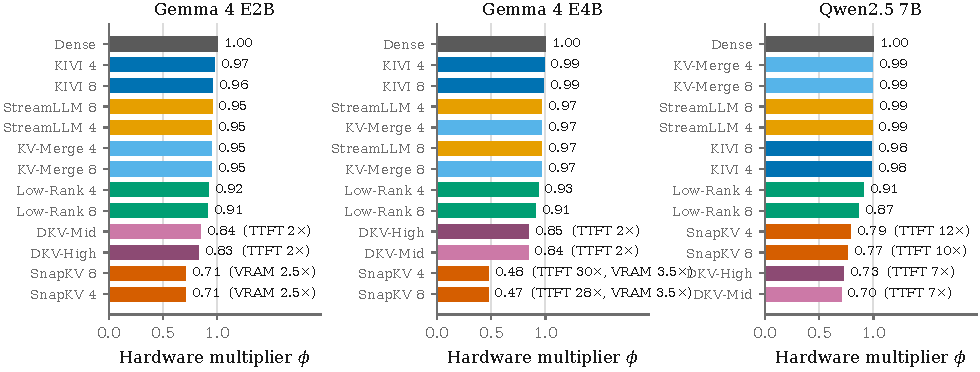
\includegraphics[width=\textwidth]{figures/fig6_hardware.pdf}
\caption{\textbf{Where the hardware multiplier is lost.} $\phi$ for every operating point, annotated with the dominant cause when a method falls materially below the dense reference. The losses are prefill-driven (SnapKV on E4B and 7B, DKV on 7B) or peak-memory-driven (SnapKV on E2B), and in no case are they predictable from the method's position in Figure~\ref{fig:effective_bits}.}
\label{fig:hardware}
\end{figure}

\subsection{Joint view: the two tracks side by side}

Figure~\ref{fig:part1} gives the Part~1 ordering and Figure~\ref{fig:hardware} the hardware term. Read together they support a modest, well-supported summary rather than a universal ranking. On these three models, under these implementations and on this hardware: grouped 4-bit quantisation is the only family that is simultaneously near the top of Axis~2 and essentially free on Axis~3 ($\phi \ge 0.97$ everywhere); eviction with observation pooling is competitive on Axes~1 and~2 and is the most expensive method we measured on Axis~3; pooling and streaming-window methods are cheap on Axis~3 and lose the most on Axis~2; and factorised representations sit in between on all three, with the largest metadata correction. We state these as findings about what we evaluated, not as properties of the method families in general.

\begin{figure}[t]
\centering
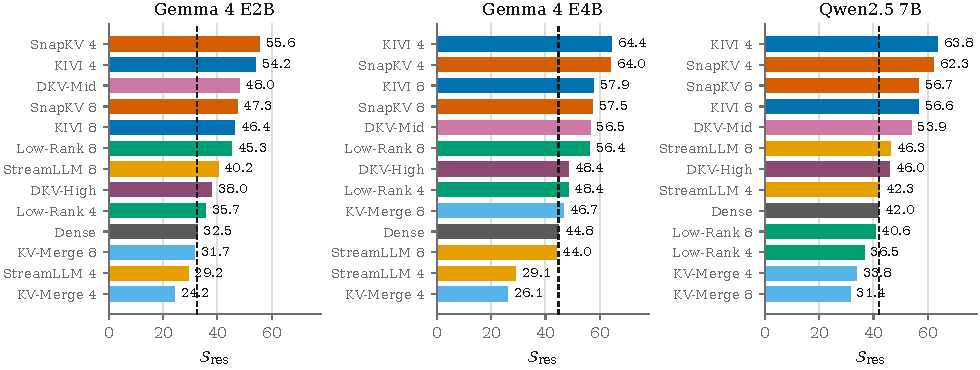
\includegraphics[width=\textwidth]{figures/fig5_part1.pdf}
\caption{\textbf{Part 1 algorithmic utility ($\Sres$) at every operating point,} with the dense reference marked (dashed). Note that dense is not last: at $\alpha = 0.70$, a method that gives up a few accuracy points for a $70\%$ memory saving outscores it.}
\label{fig:part1}
\end{figure}

\subsection{Task structure, and where the limit is the model}
\label{sec:res_tasks}

Figure~\ref{fig:heatmap} breaks accuracy down by task. Two observations bear on how the headline averages should be read.

\emph{Variable tracking is a base-model limit, not a compression effect.} Every method scores $0.0\%$ on RULER multi-step variable tracking on all three models --- including the uncompressed dense reference (a single KIVI configuration on Qwen2.5~7B reaches $3.3\%$). Whatever is failing here is not the representation. Because this task is one of five, it depresses every reported average by roughly a fifth uniformly; it does not change any ranking, but absolute accuracies in this paper should be read with it in mind.

\emph{Multi-needle retrieval is near a scoring floor for the dense reference.} Dense accuracy on multi-needle is $32$--$33\%$ on all three models, consistent with partial credit for locating a subset of the planted needles. It therefore has limited headroom to discriminate between methods. The discriminative signal in our suite comes principally from single-needle retrieval, RULER key--value lookup and multi-hop QA, where dense ranges from $80\%$ to $100\%$ and compressed methods separate cleanly.

\begin{figure}[t]
\centering
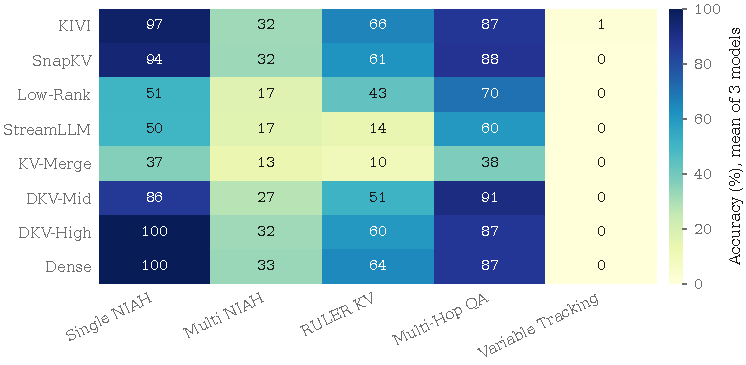
\includegraphics[width=0.76\textwidth]{figures/fig7_task_heatmap.pdf}
\caption{\textbf{Accuracy by task,} averaged over the three models and both budget levels. Variable tracking is at zero for every method \emph{and} for the uncompressed dense reference, identifying it as a base-model limitation rather than a compression failure.}
\label{fig:heatmap}
\end{figure}

\subsection{Context scaling and the quality--memory frontier}

Figure~\ref{fig:context} traces the full $2$K--$128$K ladder on Gemma~4 E2B. Dense accuracy is flat to $32$K, falls at $64$K and drops sharply at $128$K; the better compressed methods track it closely throughout, and the gap between methods does not widen systematically with context. The degradation beyond $64$K is therefore shared with the uncompressed baseline and is a property of the model's usable context, not of compression.

Figure~\ref{fig:pareto} plots the quality--memory frontier within each model. We compute the frontier per model rather than pooling: accuracy differences between a 2B and a 7B model reflect base-model capability, and a frontier drawn across them would be an artefact. The frontiers are short --- on Gemma~4 E2B a single $4$-bit configuration dominates everything else, matching dense accuracy at a quarter of the bits --- which is itself informative about how much headroom remains at these scales.

\begin{figure}[t]
\centering
\begin{minipage}[t]{0.46\textwidth}
\centering
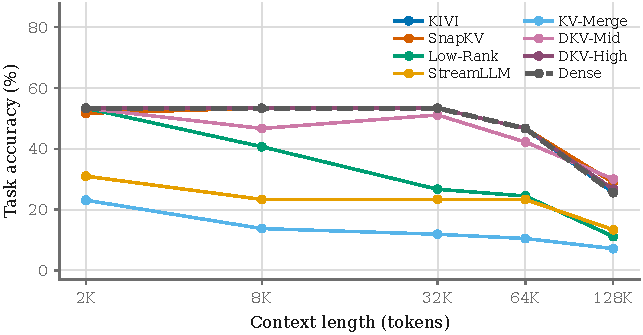
\includegraphics[width=\linewidth]{figures/fig8_context_scaling.pdf}
\caption{\textbf{The $2$K--$128$K ladder on Gemma~4 E2B.} The cliff beyond $64$K is shared with the dense reference.}
\label{fig:context}
\end{minipage}\hfill
\begin{minipage}[t]{0.52\textwidth}
\centering
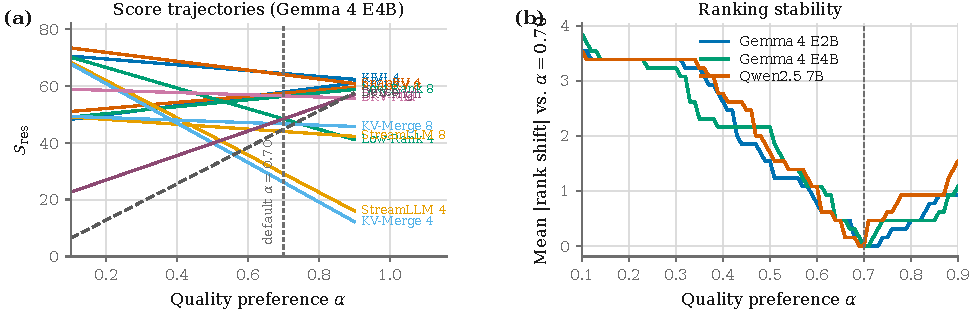
\includegraphics[width=\linewidth]{figures/fig10_alpha_sensitivity.pdf}
\caption{\textbf{Sensitivity to $\alpha$.} Score trajectories and mean rank displacement relative to the default $\alpha = 0.70$.}
\label{fig:alpha}
\end{minipage}
\end{figure}

\begin{figure}[t]
\centering
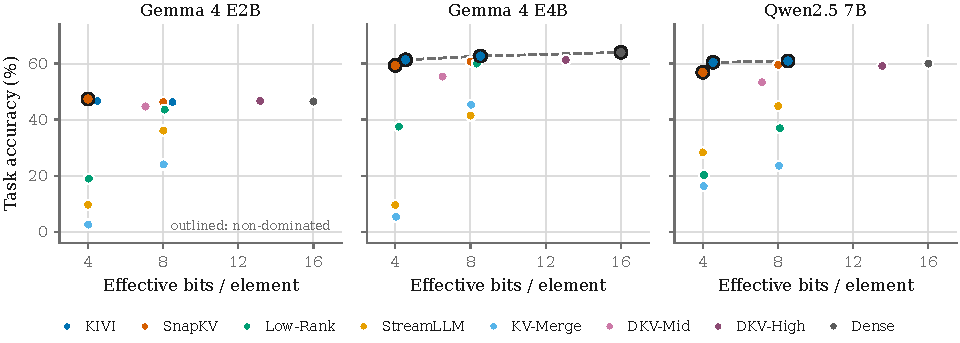
\includegraphics[width=\textwidth]{figures/fig9_pareto.pdf}
\caption{\textbf{Quality--memory frontier, computed within each model.} Effective bits include metadata. Outlined markers are non-dominated. Frontiers are not drawn across models, because accuracy differences between models reflect base-model capability rather than the representation.}
\label{fig:pareto}
\end{figure}

% =============================================================================
\section{Discussion}
\label{sec:discussion}

\paragraph{For method authors: report three numbers, not two.} The minimum honest summary of a KV-compression method is its effective bits per element \emph{including} metadata, its task accuracy against a paired dense run of the same model, and its measured TTFT, throughput and peak memory relative to that same run. Our results show each of the three carries information the other two do not. Reporting a nominal bit-width understates real footprint by $6$--$28\%$ in a method-dependent way; reporting a compression ratio without task measurement leaves an $18.7\times$ accuracy range undetermined; reporting both without a systems measurement leaves a $30\times$ latency range undetermined.

\paragraph{For practitioners: the choice depends on which axis binds.} If the binding constraint is context length in a fixed memory budget, Axis~1 with honest metadata accounting is the right selector. If it is answer quality, Axis~2 must be measured on the target model, because the ordering of methods changed between our three models. If it is interactive latency or serving cost, only Axis~3 is decisive, and it must be measured on the implementation that will actually be deployed --- our own SnapKV and DKV measurements are the clearest illustration of how far an integration can sit from an algorithm's potential.

\paragraph{For benchmark design: keep the tracks apart.} It is tempting to collapse everything into one number. We report $\Sres$ and $\Ssys$ separately, and we decline to average them into a headline, because the disagreement between them is the finding. A single score would have concealed that a configuration ranked second on representation utility ranks tenth on serving utility.

\paragraph{An honest note on our own method.} One of the evaluated families (DKV) is the authors' own prior work, and it is the family this paper's accounting penalises most. Charging it for metadata moves DKV-Mid from $5.00$ to $6.51$ effective bits per element on Gemma~4 E4B and costs it two rank positions; DKV-High loses a position on the other two models; and on the serving track the prefill cost of the block compressor leaves both configurations mid-table or lower. DKV remains above the dense reference on Part~1, which we state because it is what the numbers show, but it wins nothing here. We regard this as evidence that the instrument is doing its job rather than as a result to be softened.

% =============================================================================
\section{Scope and Limitations}
\label{sec:limitations}

We state these as constraints on what our evidence supports, not as future work.

\begin{enumerate}[leftmargin=*,itemsep=2.5pt,topsep=3pt]
    \item \textbf{Implementation, not algorithm.} Axis~3 measures code paths. Where an upstream fused kernel was unavailable on our platform --- SnapKV's patched attention, DKV's paged Triton runtime --- our numbers characterise the integration that ran, and must not be read as upper bounds on those algorithms. Table~\ref{tab:provenance} states this per method. This limitation is intrinsic to serving measurement rather than incidental to our setup: there is no implementation-independent serving number.
    \item \textbf{Analytic versus realised savings.} For KIVI and Low-Rank KV the footprint is analytically accounted while values are retained in a wider dtype, so their Part~1 savings are exact for the scheme but no device memory was freed; their favourable $\phi$ reflects that the transform is cheap, not that a production integer kernel would be. For SnapKV, StreamingLLM and KV-Merging the cache physically shrinks and both tracks are measured end to end.
    \item \textbf{Three models, two families, 2B--7B.} All conclusions are scoped to Gemma~4 E2B/E4B and Qwen2.5~7B. Method orderings already differ across these three, which is itself a reason not to extrapolate to 13B+ or 70B+ models, to different attention layouts, or to other tokenisers.
    \item \textbf{Single-GPU, single-stream.} One RTX 4070 SUPER, batch size one, no tensor or pipeline parallelism, no continuous batching, no paged attention. Multi-tenant serving changes the memory--latency trade-off substantially, and our Axis~3 conclusions do not transfer to it unexamined.
    \item \textbf{Synthetic, retrieval-weighted tasks.} Our suite probes retrieval, associative lookup and short multi-hop reasoning. It does not cover summarisation, open-ended generation, agentic dialogue or code, where the information a compressed cache must preserve is distributed differently. One task (variable tracking) is at floor for the base models and one (multi-needle) is near a scoring floor for the dense reference, so effectively three of five tasks carry the discriminative signal.
    \item \textbf{Statistical resolution.} Rank correlations are computed over $12$--$13$ operating points per model and $36$ pooled; they are descriptive summaries of a small sample, and we quote $p$-values only to indicate the absence of a detectable relationship, not to assert one. The matched-budget comparison in \S\ref{sec:res_axis12} is a direct observation and does not depend on them. Per-query variance is negligible under greedy decoding (\S\ref{sec:setup}), but $75$ distinct queries per model is a small suite and per-task accuracies are correspondingly coarse.
    \item \textbf{The weights $\alpha$ and the $\phi$ exponents are conventions.} They are reported, varied (Figure~\ref{fig:alpha}) and decomposable, but they are not derived from anything. Readers with different deployment priorities should reweight from the component columns.
\end{enumerate}

% =============================================================================
\section{Conclusion}
\label{sec:conclusion}

Compression ratio, task accuracy and serving efficiency are three separate properties of a KV-cache compression method, and in our measurements none of them predicts the others. Methods matched to within $0.19$ effective bits per element differ by up to $18.7\times$ in task accuracy; methods matched on \emph{both} footprint and accuracy differ by $30\times$ in prefill latency and $3.5\times$ in peak memory; and across $36$ operating points the footprint of a representation is statistically uninformative about the hardware efficiency it realises. Charging representations for their mandatory metadata --- which the conventional accounting omits --- changes reported bitrates by $6$--$28\%$ and reorders methods, including our own.

CRBench is the instrument these findings required: paired per-query execution against a dense reference, an effective-bits accounting that includes metadata, and two deliberately unmerged tracks. We release the code, the raw per-query records and the scripts that regenerate every number and figure in this paper, so that the accounting choices we argue for can be inspected and disagreed with directly.

% =============================================================================
\subsubsection*{Broader Impact Statement}

More efficient long-context serving lowers the cost and energy of deploying large models, and makes long-context inference feasible on commodity hardware. It also carries a specific risk that this paper is directly concerned with: lossy KV compression can cause a model to silently omit facts that were present in its context. Our measurements show this failure is not visible in a compression ratio, and that at a fixed bitrate one method can retain $47\%$ of task ability where another retains $2.5\%$. In retrieval-grounded settings where correctness matters --- clinical, legal, financial --- a compression method selected on its advertised ratio may quietly drop exactly the evidence the answer depends on. We regard the practice of reporting compression ratios without paired task and systems measurement as the risk worth naming here, and the paired, decoupled reporting we describe as a partial mitigation.

% =============================================================================
\bibliographystyle{plainnat}
\begingroup
\small
\begin{thebibliography}{24}

\bibitem[Achiam et~al.(2023)]{achiam2023gpt4} Achiam, J., Adler, S., Agarwal, S., et~al. (2023). GPT-4 technical report. \textit{arXiv preprint arXiv:2303.08774}.

\bibitem[An et~al.(2023)]{an2023leval} An, C., Gong, S., Zhong, M., et~al. (2023). L-Eval: Instituting standardized evaluation for long context language models. \textit{arXiv preprint arXiv:2307.11088}.

\bibitem[Bai et~al.(2023a)]{bai2023qwen} Bai, J., Bai, S., Chu, Y., et~al. (2023a). Qwen technical report. \textit{arXiv preprint arXiv:2309.16609}.

\bibitem[Bai et~al.(2023b)]{bai2023longbench} Bai, Y., Lv, X., Zhang, J., et~al. (2023b). LongBench: A bilingual, multitask benchmark for long context understanding. \textit{arXiv preprint arXiv:2308.14508}.

\bibitem[Bai et~al.(2024)]{bai2024longbenchv2} Bai, Y., Lv, X., Zhang, J., et~al. (2024). LongBench v2: Towards deeper understanding of long context large language models. \textit{arXiv preprint arXiv:2412.15204}.

\bibitem[Brown et~al.(2020)]{brown2020language} Brown, T., Mann, B., Ryder, N., et~al. (2020). Language models are few-shot learners. In \textit{NeurIPS}, vol.~33, pp. 1877--1901.

\bibitem[Authors withheld(2026)]{chimurkar2026dkv} [Authors withheld for double-blind review] (2026). DKV: Anchor and low-rank differential KV-cache compression for scalable long-context inference. \textit{Preprint under double-blind review}.

\bibitem[DeepSeek-AI(2024)]{deepseek2024v2} DeepSeek-AI (2024). DeepSeek-V2: A strong, economical, and efficient Mixture-of-Experts language model. \textit{arXiv preprint arXiv:2405.04434}.

\bibitem[Dettmers et~al.(2022)]{dettmers2022llmint8} Dettmers, T., Lewis, M., Belkada, Y., and Zettlemoyer, L. (2022). LLM.int8(): 8-bit matrix multiplication for transformers at scale. In \textit{NeurIPS}, vol.~35, pp. 30318--30332.

\bibitem[Dong et~al.(2023)]{dong2023bamboo} Dong, Z., Tang, T., Dai, J., et~al. (2023). BAMBOO: A comprehensive benchmark for evaluating long-sequence language models. \textit{arXiv preprint arXiv:2309.13345}.

\bibitem[Ge et~al.(2023)]{ge2023model} Ge, S., Zhang, Y., Liu, L., et~al. (2023). Model tells you what to discard: Adaptive KV cache compression for LLMs. \textit{arXiv preprint arXiv:2310.01801}.

\bibitem[Hooper et~al.(2024)]{hooper2024kvquant} Hooper, C., Kim, S., Mohammadzadeh, H., et~al. (2024). KVQuant: Towards 10 million context length LLM inference with KV cache quantization. In \textit{NeurIPS}.

\bibitem[Hsieh et~al.(2024)]{hsieh2024ruler} Hsieh, C.-Y., Sun, S., Kriman, S., et~al. (2024). RULER: What's the real context size of your long-context language model? \textit{arXiv preprint arXiv:2404.06654}.

\bibitem[Kamradt(2023)]{kamradt2023needle} Kamradt, G. (2023). Needle in a haystack --- pressure testing LLMs. \textit{GitHub repository: gkamradt/LLMTest\_NeedleInAHaystack}.

\bibitem[Li et~al.(2024)]{li2024snapkv} Li, Y., Huang, Y., Yang, B., et~al. (2024). SnapKV: LLM knows what you are looking for before generation. In \textit{NeurIPS}.

\bibitem[Liu et~al.(2023)]{liu2023scissorhands} Liu, Z., Desai, A., Liao, F., et~al. (2023). Scissorhands: Exploiting the persistence of importance in LLM KV cache. In \textit{NeurIPS}.

\bibitem[Liu et~al.(2024)]{liu2024kivi} Liu, Z., Yuan, J., Jin, H., et~al. (2024). KIVI: A tuning-free asymmetric 2-bit quantization for KV cache. In \textit{ICML}.

\bibitem[Reid et~al.(2024)]{reid2024gemini} Reid, M., Savinov, N., Teplyashin, D., et~al. (2024). Gemini 1.5: Unlocking multimodal understanding across millions of tokens of context. \textit{arXiv preprint arXiv:2403.05530}.

\bibitem[Sharma et~al.(2024)]{sharma2023truth} Sharma, P., Ash, J.~T., and Misra, D. (2024). The truth is in there: Improving reasoning in language models with layer-selective rank reduction. In \textit{ICLR}.

\bibitem[Touvron et~al.(2023)]{touvron2023llama} Touvron, H., Lavril, T., Izacard, G., et~al. (2023). LLaMA: Open and efficient foundation language models. \textit{arXiv preprint arXiv:2302.13971}.

\bibitem[Vaswani et~al.(2017)]{vaswani2017attention} Vaswani, A., Shazeer, N., Parmar, N., et~al. (2017). Attention is all you need. In \textit{NeurIPS}, vol.~30, pp. 5998--6008.

\bibitem[Xiao et~al.(2023)]{xiao2023streamingllm} Xiao, G., Tian, Y., Chen, B., et~al. (2023). Efficient streaming language models with attention sinks. In \textit{ICLR}.

\bibitem[Zhang et~al.(2023)]{zhang2023h2o} Zhang, Z., Sheng, Y., Zheng, T., et~al. (2023). $\text{H}_2\text{O}$: Heavy-hitter oracle for efficient generative inference of large language models. In \textit{NeurIPS}.

\bibitem[Zhang et~al.(2024a)]{zhang2024pyramidkv} Zhang, Y., Du, X., Liu, C., et~al. (2024a). PyramidKV: Dynamic KV cache compression based on pyramid information funneling. \textit{arXiv preprint arXiv:2406.02069}.

\bibitem[Zhang et~al.(2024b)]{zhang2024infinitebench} Zhang, X., Chen, Y., Hu, S., et~al. (2024b). $\infty$-Bench: Extending context window to 100K+ for comprehensive evaluation of LLMs. In \textit{ACL}.

\end{thebibliography}
\endgroup

\clearpage
\appendix

% =============================================================================
\section{Proof of the Scoring Properties}
\label{app:proofs}

\begin{proposition}
Let $\Sres(Q,R) = \alpha Q + (1-\alpha) R$ with $\alpha \in (0,1)$. On $[0,100]^2$, $\Sres$ is strictly increasing in each argument, bounded in $[0,100]$, and Pareto consistent.
\end{proposition}

\begin{proof}
\emph{Monotonicity}: $\partial \Sres / \partial Q = \alpha > 0$ and $\partial \Sres / \partial R = 1 - \alpha > 0$.
\emph{Boundedness}: $\Sres$ is a convex combination of $Q$ and $R$, so $\min(Q,R) \le \Sres \le \max(Q,R)$, giving $\Sres \in [0,100]$ with the extremes attained at $(0,0)$ and $(100,100)$.
\emph{Pareto consistency}: if $Q_A \ge Q_B$ and $R_A \ge R_B$ with at least one strict, then $\Sres(Q_A,R_A) - \Sres(Q_B,R_B) = \alpha(Q_A - Q_B) + (1-\alpha)(R_A - R_B) > 0$.
\end{proof}

\section{Alternative Utility Formulations}
\label{app:formulations}

We considered multiplicative ($Q^{\alpha} R^{1-\alpha}$), harmonic and threshold-gated alternatives. All satisfy monotonicity and Pareto consistency; the multiplicative and harmonic forms additionally satisfy a substitution-resistance property that the linear form does not, in that a zero on either axis annihilates the score. We chose the linear form regardless, for two reasons. First, annihilation is undesirable here: the dense reference has $R_{\text{mem}} = 0$ by definition and would score zero under any multiplicative form, removing the one anchor every other row is measured against. Second, a linear score can be decomposed back into its inputs by inspection, which matters more for a benchmark intended to be argued with than a marginally better-behaved aggregate would. Figure~\ref{fig:alpha} shows the ranking is stable across $\alpha$, so the choice of weight is not doing hidden work.

\section{Per-Model Detail}
\label{app:permodel}

Tables~\ref{tab:part1} and~\ref{tab:part2} in the main text already list every operating point for all three models. Table~\ref{tab:matched} isolates the matched-budget comparison that supports \S\ref{sec:res_axis12}, reporting the three models side by side at each nominal budget.

\begin{table}[h]
\centering
\small
\setlength{\tabcolsep}{5.5pt}
\caption{\textbf{Matched nominal budget across models.} Accuracy per model at each controlled budget, with the mean realised $\beff$, mean TTFT inflation against the paired dense run, and mean hardware multiplier. Within a block every method holds the same nominal budget, so accuracy differences are attributable to how the budget is spent.}
\label{tab:matched}
\begin{tabular}{l ccc ccc}
\toprule
\textbf{Method} & \textbf{E2B} & \textbf{E4B} & \textbf{7B} & $b_{\text{eff}}$ & \textbf{TTFT $\times$dense} & $\phi$ \\
\midrule
\multicolumn{7}{l}{\textit{Nominal budget: 4~bits/element}} \\
\midrule
KIVI (INT4/INT8) & 46.7\% & 61.3\% & 60.4\% & 4.54 & 1.00$\times$ & 0.98 \\
SnapKV & 47.3\% & 59.3\% & 56.9\% & 4.01 & 14.36$\times$ & 0.66 \\
Low-Rank KV & 18.9\% & 37.5\% & 20.2\% & 4.11 & 1.10$\times$ & 0.92 \\
StreamingLLM & 9.6\% & 9.5\% & 28.3\% & 4.01 & 1.01$\times$ & 0.97 \\
KV-Merging & 2.5\% & 5.3\% & 16.2\% & 4.04 & 1.01$\times$ & 0.97 \\
\midrule
\multicolumn{7}{l}{\textit{Nominal budget: 8~bits/element}} \\
\midrule
KIVI (INT4/INT8) & 46.2\% & 62.7\% & 60.9\% & 8.52 & 1.00$\times$ & 0.98 \\
SnapKV & 46.2\% & 60.7\% & 59.6\% & 8.01 & 13.08$\times$ & 0.65 \\
Low-Rank KV & 43.6\% & 60.0\% & 36.9\% & 8.18 & 1.16$\times$ & 0.90 \\
StreamingLLM & 36.1\% & 41.4\% & 44.8\% & 8.01 & 1.01$\times$ & 0.97 \\
KV-Merging & 24.0\% & 45.3\% & 23.5\% & 8.04 & 1.01$\times$ & 0.97 \\
\bottomrule
\end{tabular}

\end{table}

\section{Measurement Protocol}
\label{app:protocol}

\paragraph{Execution.} Prefill is executed in $4{,}096$-token chunks. The context transform is applied to the resident PyTorch KV cache after prefill (or streaming during prefill, for the quantiser), and generation proceeds from the transformed cache. Decoding is greedy. TTFT is measured with device synchronisation around the full prefill-plus-transform-plus-first-token path, so transform cost is charged to the method that incurs it. Peak device memory is the maximum allocated over the whole query.

\paragraph{What is charged to metadata.} Quantisation scales and zero points; SVD factor matrices; DKV anchor and basis state; 32-bit token position indices for eviction methods; and dtype-alignment padding where the scheme requires it. Partial groups that cannot be quantised at the target width are charged at 16 bits.

\paragraph{Reproduction.} The scripts under \texttt{paper/analysis/} regenerate, in order, every number in the tables (\texttt{build\_tables.py}), every statistic quoted in \S\ref{sec:results} (\texttt{decoupling\_analysis.py}), and every figure (\texttt{make\_figures.py}), reading only the released per-query records in \texttt{results/<model>/progress.jsonl}. A fourth script, \texttt{verify\_claims.py}, re-derives each quantity quoted in the prose from those outputs and asserts that the manuscript source contains the matching value; it exits non-zero on any drift. No number in this paper is transcribed by hand.

\end{document}
